\documentclass{article}
\usepackage{amsmath}
\usepackage[mathletters]{ucs}
\usepackage[utf8x]{inputenc}
\usepackage[margin=1.5in]{geometry}
\usepackage{enumerate}
\newtheorem{theorem}{Theorem}
\usepackage[dvipsnames]{xcolor}
\usepackage{pgfplots}
\pgfplotsset{compat=1.18}
\setlength{\parindent}{0cm}
\usepackage{graphics}
\usepackage{graphicx} % Required for including images
\usepackage{subcaption}
\usepackage{bigintcalc}
\usepackage{pythonhighlight} %for pythonkode \begin{python}   \end{python}
\usepackage{appendix}
\usepackage{arydshln}
\usepackage{physics}
\usepackage{booktabs} 
\usepackage{adjustbox}
\usepackage{mdframed}
\usepackage{relsize}
\usepackage{physics}
\usepackage[thinc]{esdiff}
\usepackage{esint}  %for lukket-linje-integral
\usepackage{xfrac} %for sfrac
\usepackage{hyperref} %for linker, må ha med hypersetup
\usepackage[noabbrev, nameinlink]{cleveref} % to be loaded after hyperref
\usepackage{amssymb} %\mathbb{R} for reelle tall, \mathcal{B} for "matte"-font
\usepackage{listings} %for kode/lstlisting
\usepackage{verbatim}
\usepackage{graphicx,wrapfig,lipsum,caption} %for wrapping av bilder
\usepackage{mathtools} %for \abs{x}
\usepackage[norsk]{babel}
\usepackage{cancel}
\definecolor{codegreen}{rgb}{0,0.6,0}
\definecolor{codegray}{rgb}{0.5,0.5,0.5}
\definecolor{codepurple}{rgb}{0.58,0,0.82}
\definecolor{backcolour}{rgb}{0.95,0.95,0.92}
\lstdefinestyle{mystyle}{
    backgroundcolor=\color{backcolour},   
    commentstyle=\color{codegreen},
    keywordstyle=\color{magenta},
    numberstyle=\tiny\color{codegray},
    stringstyle=\color{codepurple},
    basicstyle=\ttfamily\footnotesize,
    breakatwhitespace=false,         
    breaklines=true,                 
    captionpos=b,                    
    keepspaces=true,                 
    numbers=left,                    
    numbersep=5pt,                  
    showspaces=false,                
    showstringspaces=false,
    showtabs=false,                  
    tabsize=2
}

\lstset{style=mystyle}
\author{Oskar Idland}
\title{Oblig 8}
\date{}
\begin{document}
\maketitle
\newpage





\section*{Problem 8.3 (H)}
\subsection*{a)}

The two lowest shells are completely filled, which in general means having $L = S = 0$. We therefore only look at the p-shells. They value $s = 1 / 2$ and $l = 2$
\[
S_{\text{tot}} = \left\{0,1\right\} \quad , \quad L_{\text{tot}} = \left\{0,1,2\right\}
\]
Creating combinations with these values we discard the symmetrical ones, as electrons are fermions. These states $(L,S)$are therefore:
\[
(0, 0), (1,1), (2,0)
\]
This gives us three possible total spin $J ∈ \left\{0,1,2\right\}$. 
Using the term symbol notation to describe these states we get:
\[
^1S_0 \ ,\ ^3P_0 \ ,\ ^3P_1 \ ,\  ^3P_2 \ ,\ ^1D_2 
\]

\subsection*{b)}
Hunds rules says the lowest energy state is the one with the highest $S$ value. This is all the $P$, states. Hunds rule also specifies that for a given degeneracy the lowest energy state belongs to the state with the lowest total angular momentum $J$. This is the $^3P_0$ state. : 
\[
^3P_0
\]


\newpage
\section*{Problem 8.4 (H)}
\subsection*{a}
Plotting the equation for a range of $z$-values to find the values $z_0$. Using this we can solve the equation using scipy. 
\subsection*{b)}
\begin{figure}[h!]
\centering
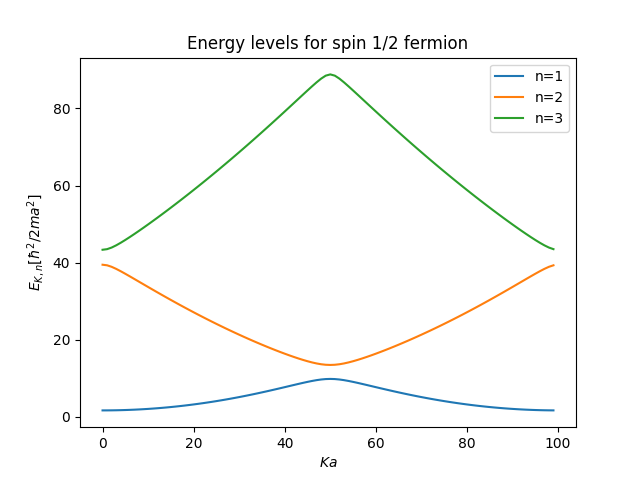
\includegraphics[width = .65\textwidth]{8.4.png}
\caption{}
\label{fig: 8.4}
\end{figure} 

\subsection*{c)}
As there is space for $2N$ electrons in each shell, we know that with $3N$ electrons the lowest shell is filled, and the one above is half-filled. We find the lowest energy by filling the lowest energy level of the second shell. The fermi wave vectors are therefore $K_f = π / 2$ and $K_f = 3π / 2$. which occur at $l = 25$ and $l = 75$ respectively. The fermi energy is therefore $E_f ≈ 24$


\section*{Problem 8.5 (H)}
\subsection*{a)}
The total energy of a harmonic oscillator is given by:
\[
E_n = ℏ ω \left(n + \frac{1}{2}\right) \quad , \quad n = 0,1,2,3...
\]
With a two-dimensional harmonic oscillator we have:
\[
E_n = E_{n_1} + E_{n_2} = ℏω(n_1 + n_2 + 1) 
\]
Representing a state using $\ket{n_1n_2}$. We obviously see the lowest energy is in the state $\ket{00}$. Next we have $\ket{10}$ and $\ket{01}$, which have the same energy. The two lowest energy states are therefore $ℏω$, $2ℏω$ where the latter has a degeneracy of two. The third-lowest level energy levels belongs to $\ket{11}$, $\ket{20}$ and $\ket{02}$ with energy $3ℏω$ and a degeneracy of three. 

\subsection*{b)}
\begin{tabular}{ c|r }
$n$ &$E_n / n$ \\
\hline
1 &1 \\
2 &1 \\
3 &4 / 3 \\
4 &6 / 4 \\
5 &8 / 5 \\
6 &10 / 6 \\
7 &13 / 7 \\
\end{tabular}

\subsection*{c)}
Inert elements are defined as an element where adding an electron makes the energy per particle to jump. We see this occurs at $n = 2, 6, 12, \ldots$ which continues to make jumps of 6. 

\begin{figure}[h!]
\centering
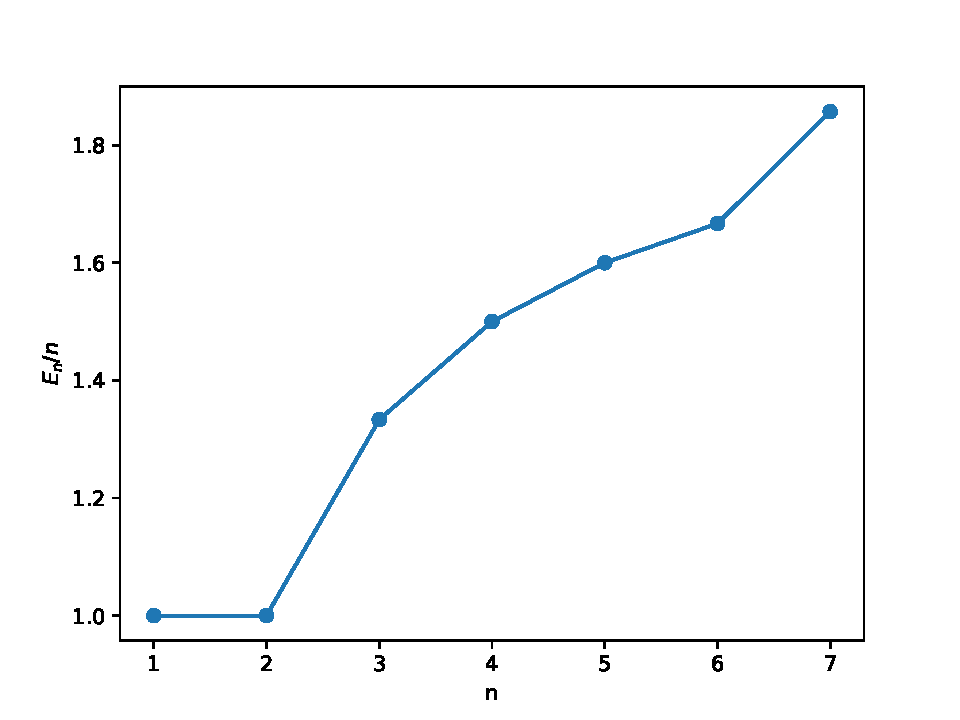
\includegraphics[width = .85\textwidth]{8.5.pdf}
\caption{Plot of the energy per number of particles in the two-dimensional harmonic oscillator.}
\label{fig: 8.5}
\end{figure}



\end{document}